\onecolumn
%\usepackage{MnSymbol}
%\usepackage{catchfilebetweentags}
%
\newcommand{\I}{\mathcal{I}}
\newcommand{\M}{\mathcal{M}}
\newcommand{\timestr}{\mathcal{T}}

\newcommand{\D}{\mathcal{D}}
\newcommand{\C}{\mathcal{C}}

%old, compatibility reasons
\newcommand{\U}{\mathbf{U}}
\newcommand{\Snc}{\mathbf{S}}
\newcommand{\T}{\mathbf{T}}
\newcommand{\R}{\mathbf{R}}

\newcommand{\Nat}{\mathbb{N}}
\newcommand{\Z}{\mathbb{Z}}
\newcommand{\Real}{\mathbb{R}}
\newcommand{\Q}{\mathbb{Q}}

%old, compatibility reasons

\newcommand{\X}[1]{\mathbf{X}\left(#1\right)}
\newcommand{\Y}[1]{\mathbf{Y}\left(#1\right)}

%\newcommand{\X}{\mathbf{X}}
%\newcommand{\Y}{\mathbf{Y}}


\newcommand{\Zed}{\mathbf{Z}}
\newcommand{\Lng}{\mathscr {L}}
\newcommand{\iFF}{\Leftrightarrow}
\newcommand{\niFF}{\nLeftrightarrow}
\newcommand{\SNC}{{\mathcal S}}
\newcommand{\TRG}{{\mathcal T}}
\newcommand{\zot}{$\mathds{Z}$ot}
%old, compatibility reasons
\newcommand{\G}[1]{\mathbf{G}\left(#1\right)}
\newcommand{\F}[1]{\mathbf{F}\left(#1\right)}
%\newcommand{\Q}{\mathbb{Q}}

\newcommand{\triple}[3]{(#1, #2, #3)}
\newcommand{\pair}[2]{(#1, #2)}
\newcommand{\siff}{\Leftrightarrow}
\newcommand{\A}{\mathcal{A}}
\newcommand{\aX}{\mathrm{X}}
\newcommand{\aY}{\mathrm{Y}}
\newcommand{\x}{\mathbf{x}}
\newcommand{\eqdef}{\stackrel{\mbox{\begin{tiny}def\end{tiny}}}{=}} % =def=
\newcommand{\iFFdef}{\stackrel{\mbox{\begin{tiny}def\end{tiny}}}{\iFF}}
% =def=
\newcommand{\step}[1]{\xrightarrow{#1}}

\newcommand{\pspace}{\textsc{PSpace}}


\makeatletter
\def\Eqlfill@{\arrowfill@\Relbar\Relbar\Relbar}
\newcommand{\longmodels}[1][]{\,|\!\!\!\ext@arrow 0359\Eqlfill@{#1}}
\makeatother

\newcommand{\symodels}{\longmodels{\mbox{\it{\tiny sym}}}}

\newcommand{\intervaLii}[2]{[#1,#2]}
\newcommand{\intervaLie}[2]{[#1,#2)}
\newcommand{\intervaLee}[2]{(#1,#2)}

\newcommand{\interval}[2]{\langle #1,#2 \rangle}

\newcommand{\set}[1]{\{ #1 \}}

\newcommand{\tsys}[1]{\mathcal{S}(#1)}


\newcommand{\lapp}[1]{\lfloor #1 \rfloor}
\newcommand{\happ}[1]{\lceil #1 \rceil}


\newcommand{\first}[2]{(H_{#1}\vee L_{#1}) \wedge(\neg(H_{#1}\vee L_{#1}) \Snc (#2))}



\newcommand{\pname}[1]{\ensuremath{\textit{#1}}}
\newcommand{\on}{\pname{on}}
\newcommand{\off}{\pname{off}}
\newcommand{\lon}{\pname{l}}
\newcommand{\test}{\pname{test}}
\newcommand{\resetc}{\pname{reset-c}}
\newcommand{\turnoff}{\pname{turnoff}}




\newcommand{\edge}[1]{\texttt{#1}}
\newcommand{\enabled}[1]{\texttt{e}_{#1}}

\newcommand{\visit}[1]{\mathit{visit}(#1)}
\newcommand{\inv}[1]{\mathit{inv}(q_{#1})}


\newcommand{\intg}[1]{\lfloor#1\rfloor}
\newcommand{\fract}[1]{\mathit{frac(#1)}}



%%%%%%%%%%%%%%% STORM MODEL COMMANDS


\newcommand{\ori}{\mathtt{orig}}
%commands with single parameter
\newcommand{\p}[1]{\mathtt{process}_{#1}}
\newcommand{\ta}[1]{\mathtt{take}_{#1}}
\newcommand{\e}[1]{\mathtt{emit}_{#1}}
\newcommand{\add}[1]{\mathtt{add}_{#1}}
\newcommand{\f}[1]{\mathtt{fail}_{#1}}
\newcommand{\buf}[1]{\mathtt{buffer}_{#1}}
\newcommand{\startf}[1]{\mathtt{startFailure}_{#1}}
\newcommand{\startid}[1]{\mathtt{startIdle}_{#1}}
\newcommand{\id}[1]{\mathtt{idle}_{#1}}
\newcommand{\cl}[1]{\mathtt{clock}_{#1}}
\newcommand{\cltf}[1]{ \cl{to\f{#1}}}
\newcommand{\ph}[1]{\mathtt{phase}_{#1}}

%commands with two parameters (index, rate)
\newcommand{\pr}[2]{\p{#1}(#2)}
\newcommand{\tar}[2]{\ta{#1}(#2)}
\newcommand{\er}[2]{\e{#1}(#2)}
\newcommand{\addr}[2]{\add{#1}(#2)}
\newcommand{\ra}[1]{r_{\add{#1}}}
\newcommand{\rp}[1]{r_{\p{#1}}}
\newcommand{\re}[1]{r_{\e{#1}}}
\newcommand{\rt}[1]{r_{\ta{#1}}}
\newcommand{\rf}[1]{r_{\mathtt{failure}_{#1}}}
\newcommand{\rff}[2]{r_{\mathtt{failure}_{#1#2}}}
\newcommand{\rr}[1]{r_{\mathtt{replay}_{#1}}}
\newcommand{\reb}[1]{\bar{r}_{\e{#1}}}
\newcommand{\rth}[1]{\hat{r}_{\ta{#1}}}
\newcommand{\reh}[1]{\hat{r}_{\e{#1}}}

\newcommand{\tph}[2]{t_{\ph{#1}}^{#2} }

	 
%
%
%%commands with single parameter
%\newcommand{\p}[1]{\mathtt{process}_{#1}}
%\newcommand{\ta}[1]{\mathtt{take}_{#1}}
%\newcommand{\e}[1]{\mathtt{emit}_{#1}}
%\newcommand{\add}[1]{\mathtt{add}_{#1}}
%\newcommand{\f}[1]{\mathtt{fail}_{#1}}
%\newcommand{\startf}[1]{\mathtt{startFailure}_{#1}}
%\newcommand{\startid}[1]{\mathtt{startIdle}_{#1}}
%\newcommand{\id}[1]{\mathtt{idle}_{#1}}
%\newcommand{\cl}[1]{\mathtt{clock}_{#1}}
%\newcommand{\cltf}[1]{ \cl{to\f{#1}}}
%\newcommand{\ph}[1]{\mathtt{phase}_{#1}}
%
%%commands with two parameters (index, rate)
%\newcommand{\pr}[2]{\p{#1}(#2)}
%\newcommand{\tar}[2]{\ta{#1}(#2)}
%\newcommand{\er}[2]{\e{#1}(#2)}
%\newcommand{\addr}[2]{\add{#1}(#2)}
%
%\newcommand{\ra}[1]{r_{\add{#1}}}
%\newcommand{\rp}[1]{r_{\p{#1}}}
%\newcommand{\re}[1]{r_{\e{#1}}}
%\newcommand{\rt}[1]{r_{\ta{#1}}}
%\newcommand{\rf}[1]{r_{\mathtt{failure}_{#1}}}
%\newcommand{\rff}[2]{r_{\mathtt{failure}_{#1#2}}}
%\newcommand{\rr}[1]{r_{\mathtt{replay}_{#1}}}
%\newcommand{\reb}[1]{\bar{r}_{\e{#1}}}
%\newcommand{\rth}[1]{\hat{r}_{\ta{#1}}}
%
%\newcommand{\tph}[2]{t_{\ph{#1}}^{#2} }


\section{Appendix-extended results}\label{app:extended-exp-results}
\noindent
This appendix shows the some extended result of the verification tool.
We exercised on applying OSTIA-BASED formal verification to support continuous architecting of the ``focused-crawler topology''.
All the experiments were carried out with a random initial configuration for the queue occupancy which allowed us to detect possible executions leading to unbounded queues.
The three experiments were parameterized with different values of $ \alpha $ (time to process  one tuple).


%\begin{figure}[h]
%	\centering 
%	\subfigure[{\footnotesize Starting configuration of the model: All the three bolt queues show an unbounded behavior. }]{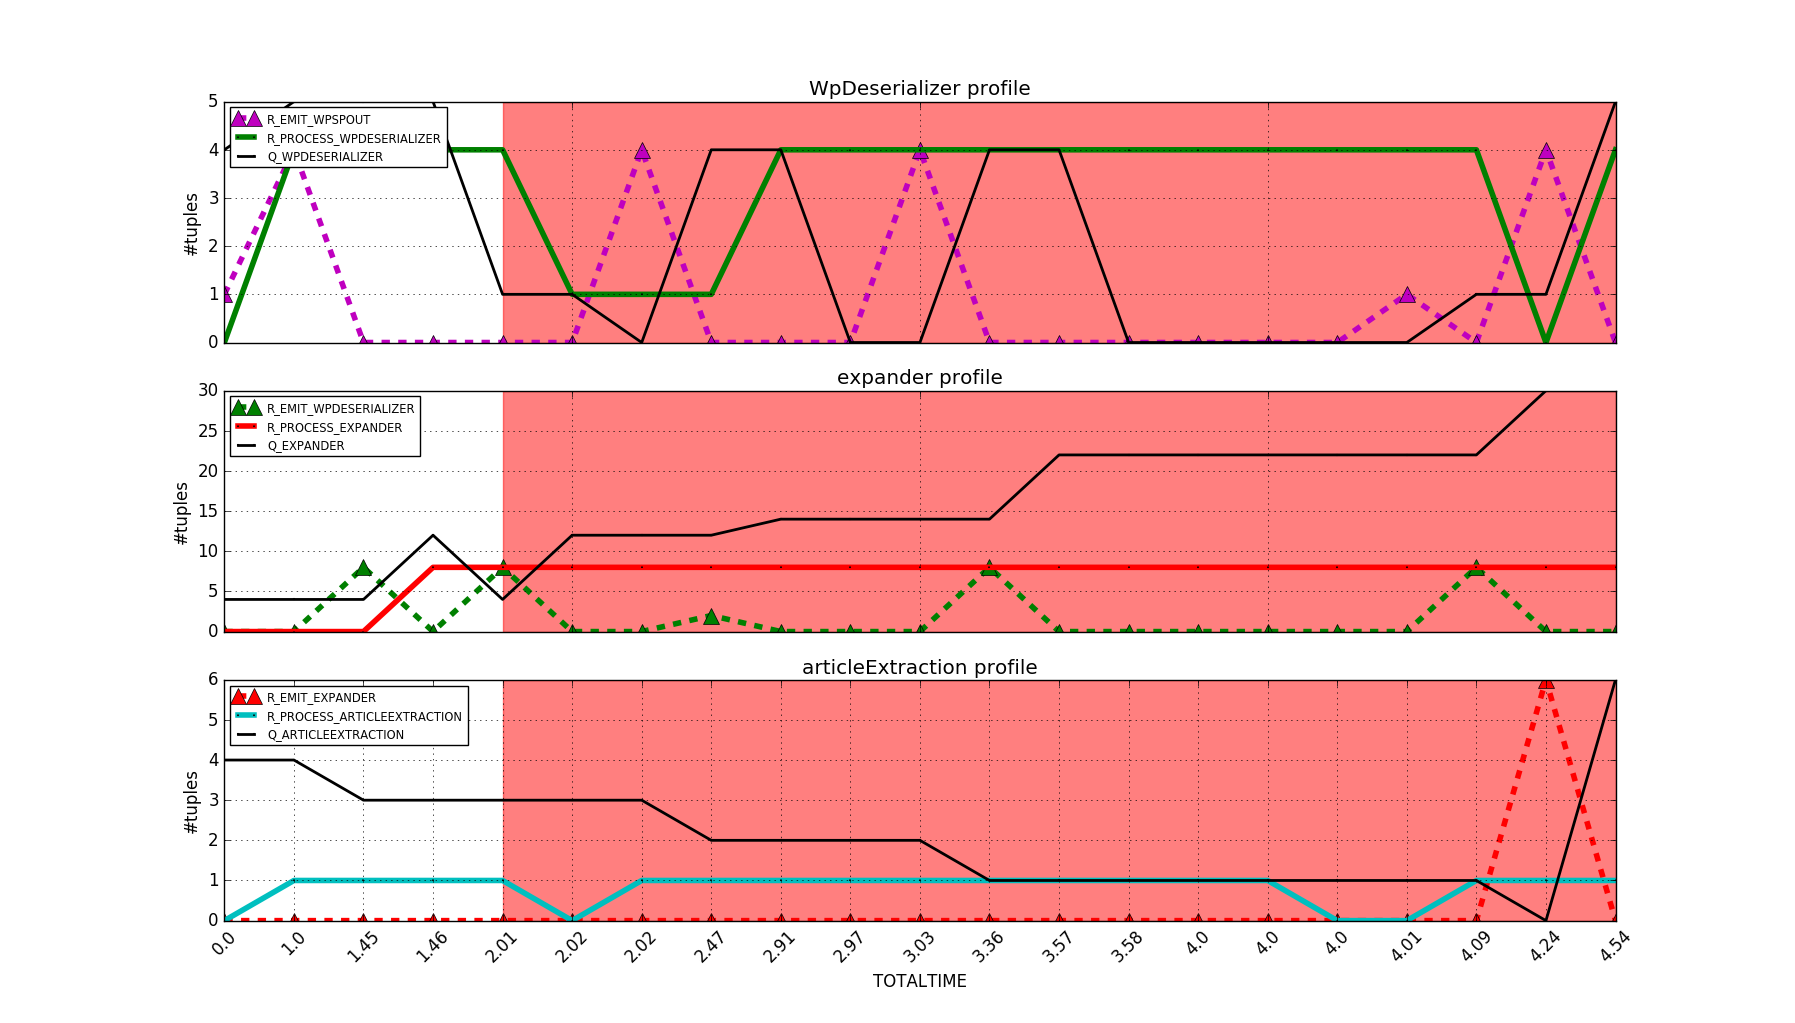
\includegraphics[width=0.45\linewidth]{images/appendix/3bolts-1}}\label{vb1}
%	\hspace{0.5cm}
%	\subfigure[{\footnotesize WpDeserializer seems to better manage the incoming tuples flow, but it still unbounded, as the other bolts.}]{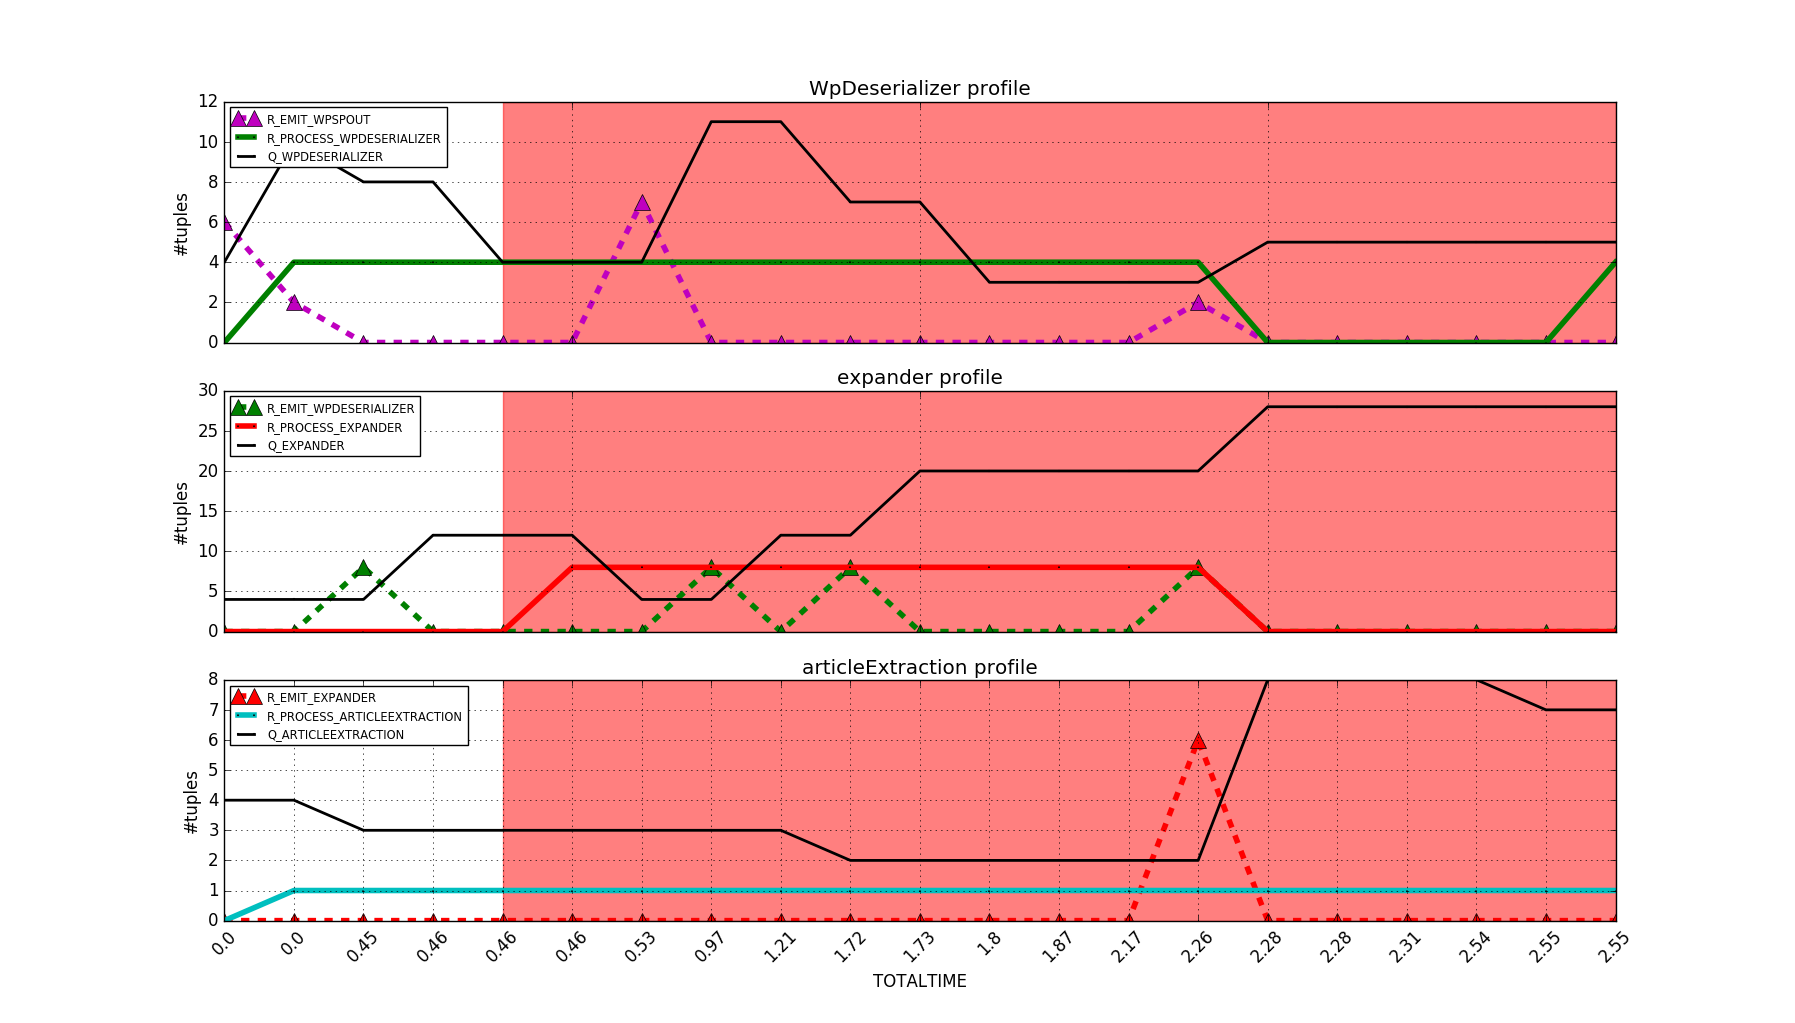
\includegraphics[width=0.45\linewidth]{images/appendix/3bolts-2}}\label{vb2}
%	%\hspace{0.5cm}
%	\subfigure[{\footnotesize This configuration allows WpDeserializer bolt to process the incoming tuple rate from the spout. Problems are still present for expander and articleExtraction }]{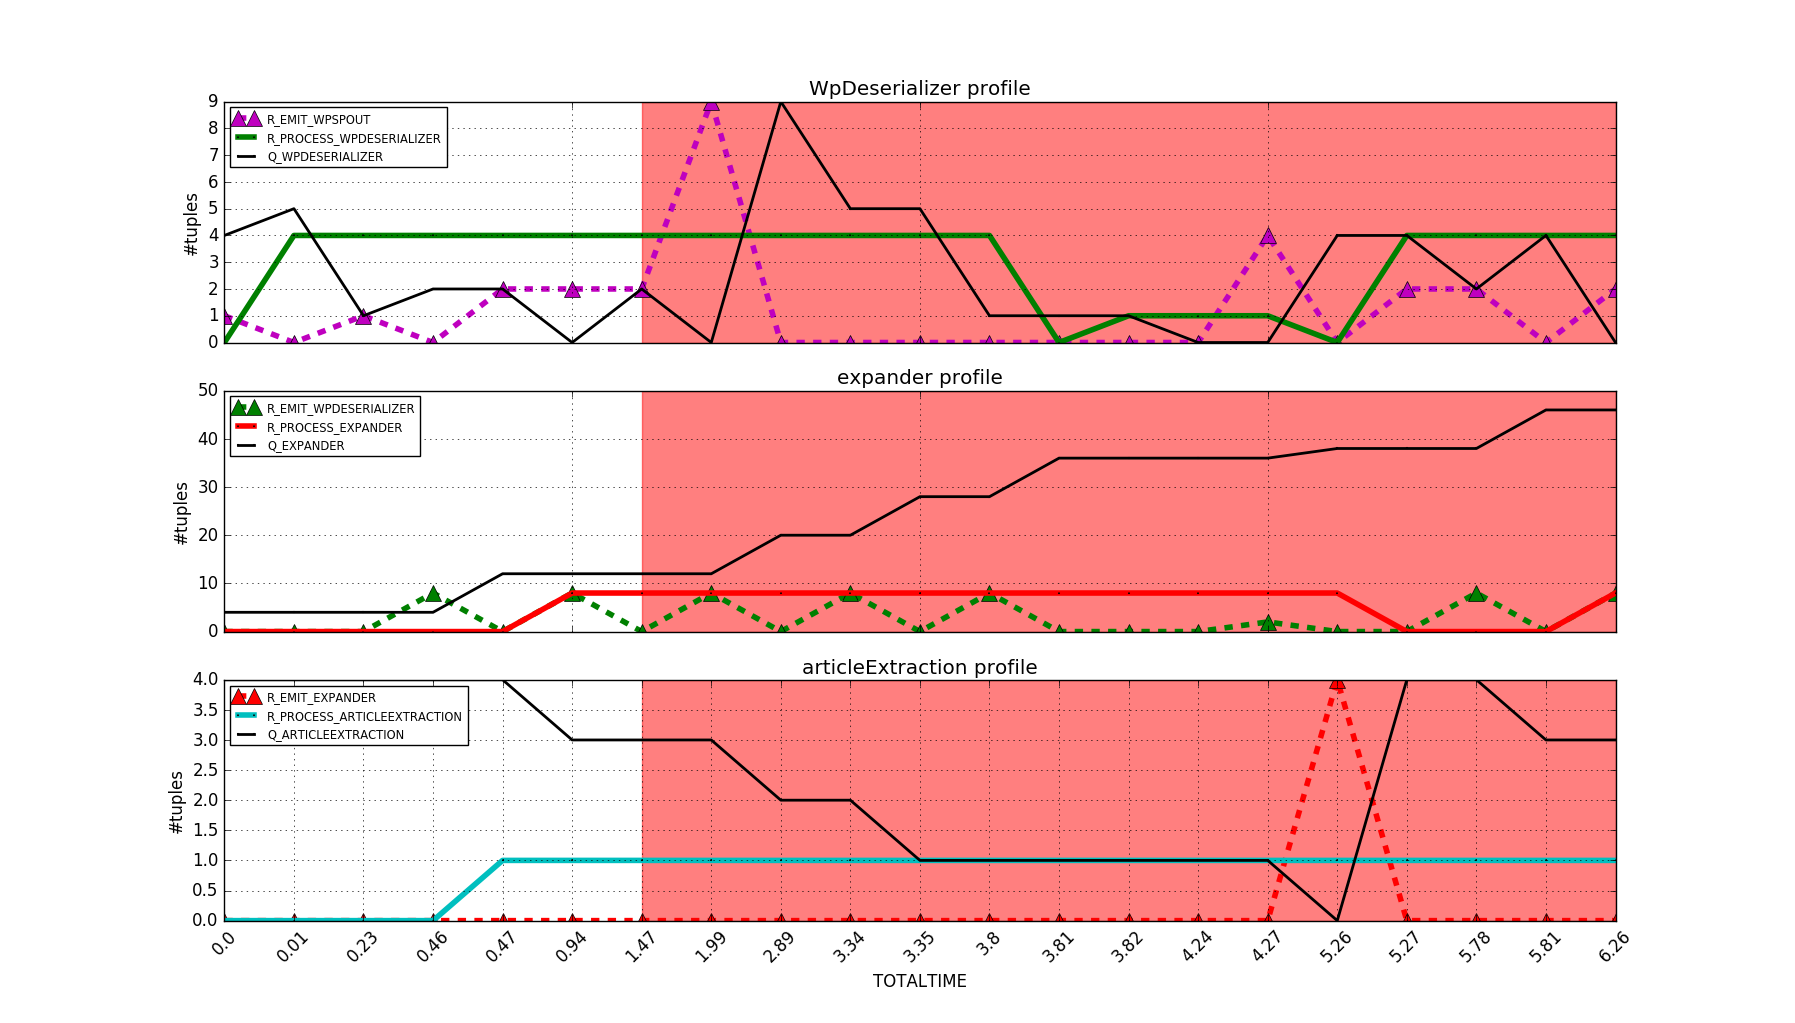
\includegraphics[width=0.45\linewidth]{images/appendix/3bolts-3}}\label{vb3}
%\end{figure}
\begin{figure}[h]
	\centering
	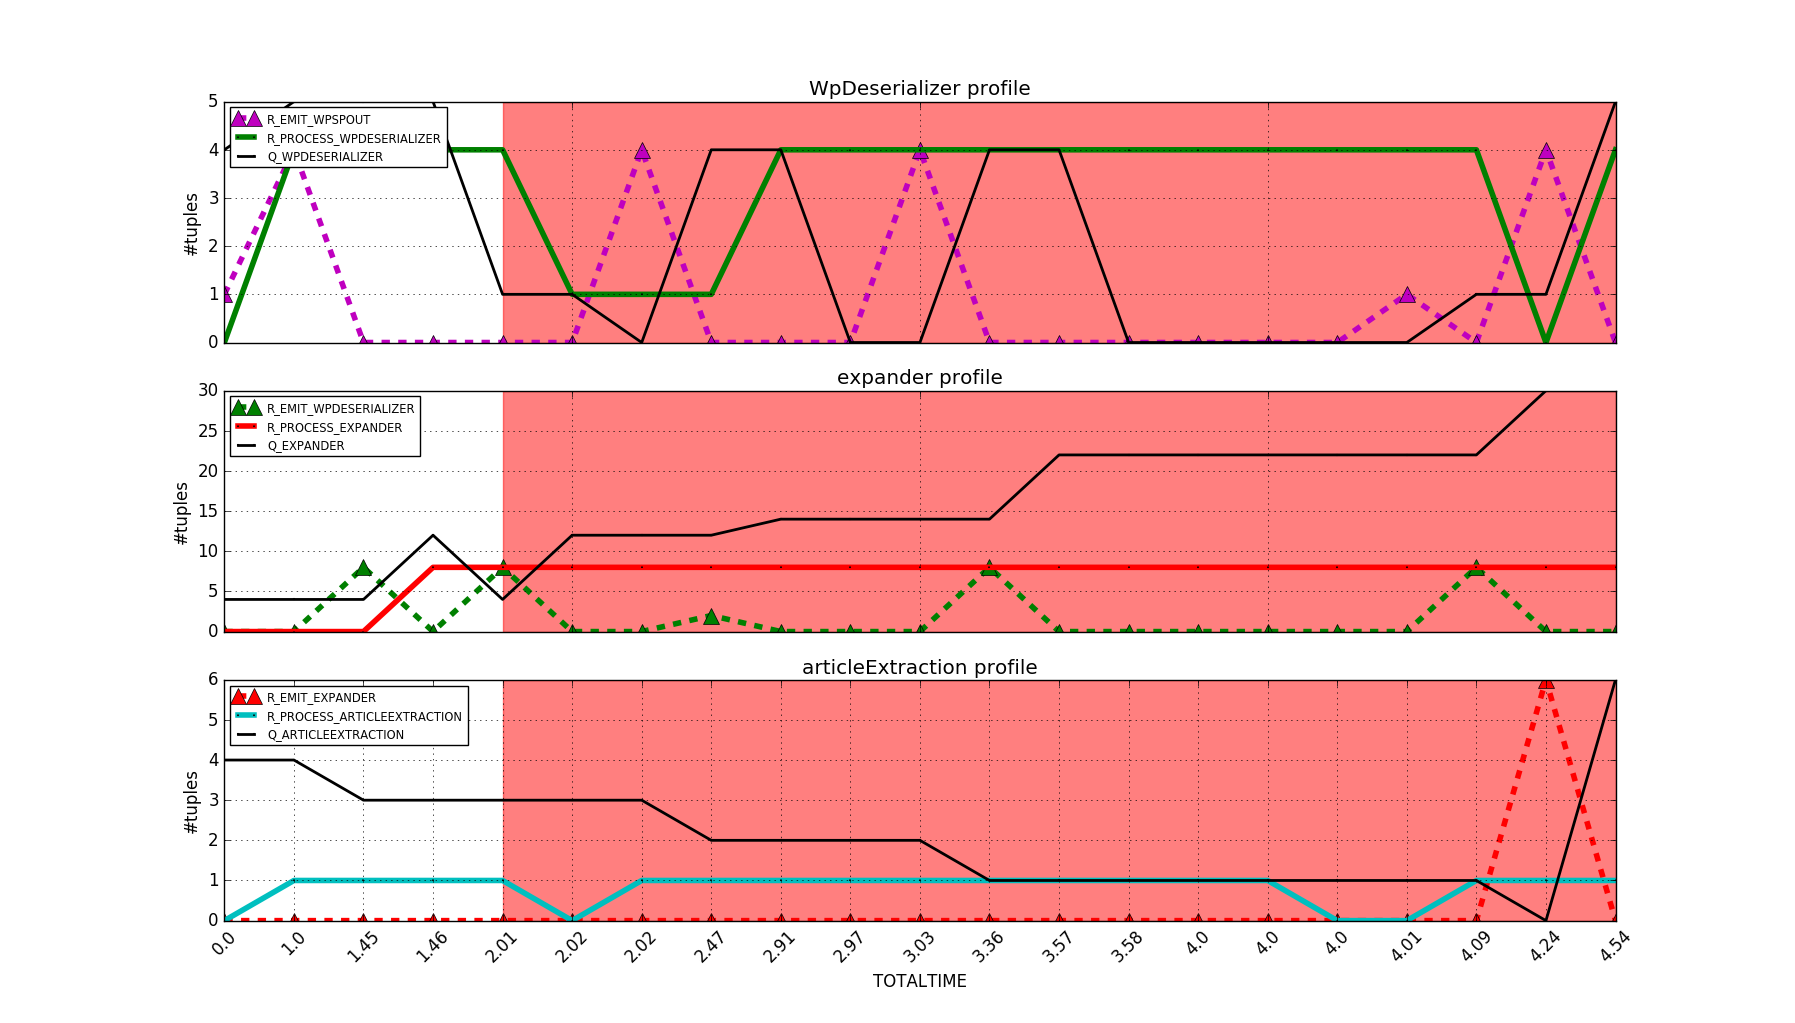
\includegraphics[width=0.7\linewidth]{images/appendix/3bolts-1}
	\caption{Starting configuration of the model: All the three bolt queues show an unbounded behavior.}
	\label{fig:3bolts-1}
\end{figure}

\begin{figure}[h]
	\centering
	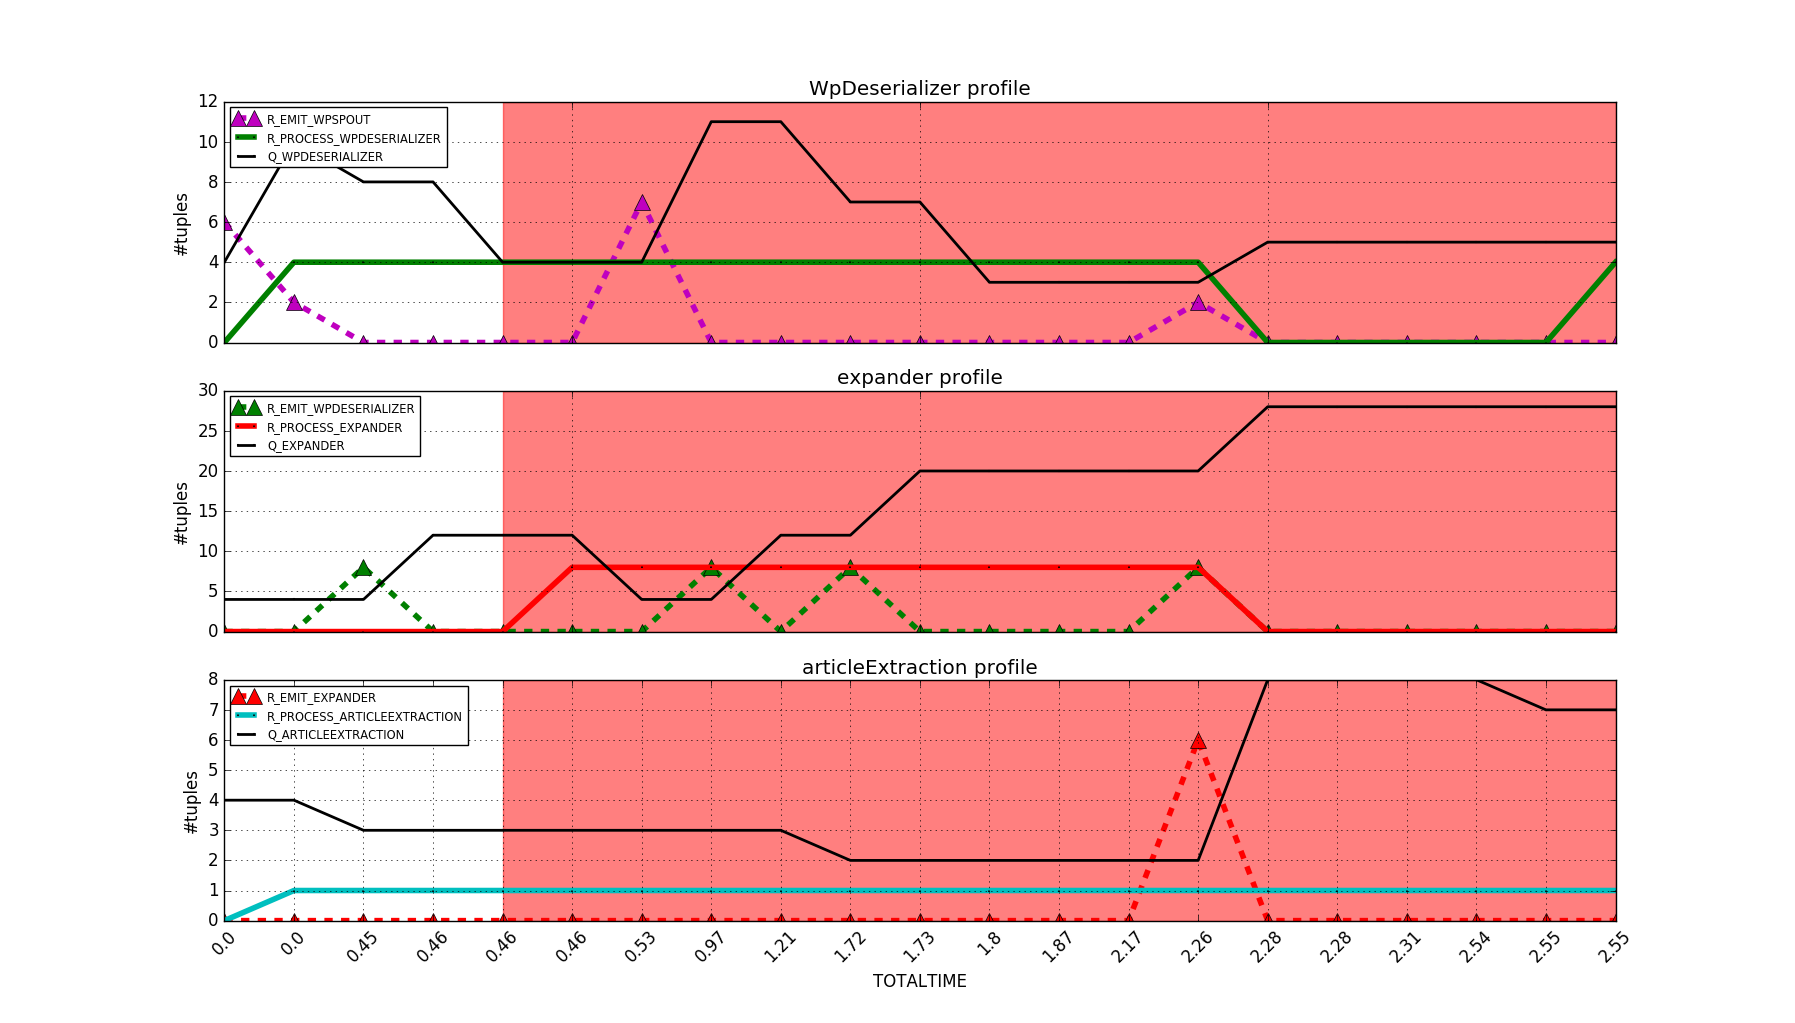
\includegraphics[width=0.7\linewidth]{images/appendix/3bolts-2}
	\caption{WpDeserializer seems to better manage the incoming tuples flow, but it still unbounded, as the other bolts.}
	\label{fig:3bolts-2}
\end{figure}

\begin{figure}[h]
	\centering
	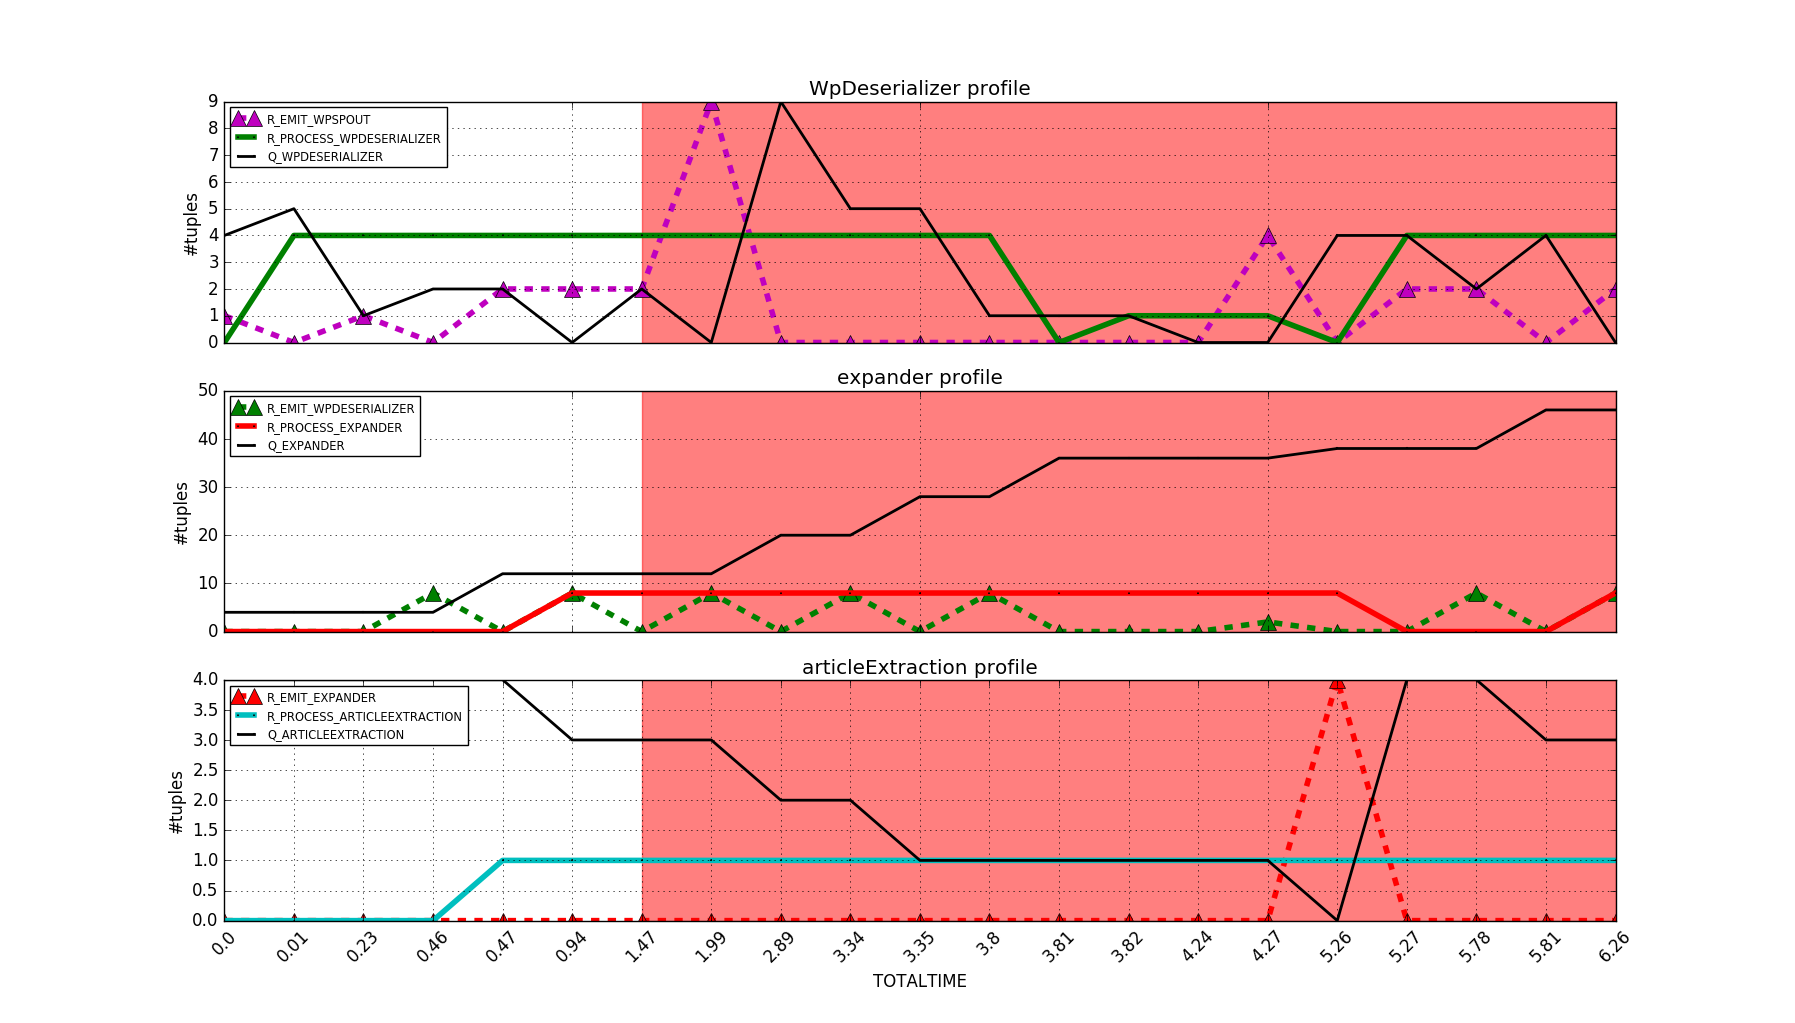
\includegraphics[width=0.7\linewidth]{images/appendix/3bolts-3}
	\caption{This configuration allows WpDeserializer bolt to process the incoming tuple rate from the spout. Problems are still present for expander and articleExtraction}
	\label{fig:3bolts-3}
\end{figure}

\clearpage
\section{Appendix-Formal model}\label{app:extended-formal-model}
\noindent
This appendix is an extract of the full CLTLoc model to provide the user with a clear overview of the formal background behind the verification in OSTIA.
Therefore, some part are missing, in particular, those related to the modeling of node failures.

A Storm topology formal definition is already given in Section~\ref{rs}.
%A Storm Topology is a directed graph $\mathbf{G} = \{ \mathbf{N}, \mathbf{E}\}$ such that the set of nodes $\mathbf{N} = \mathbf{S}\bigcup \mathbf{B}$ includes in the sets of spouts (\textbf{S}) and bolts (\textbf{B}), while the set of edges $\mathbf{E} = \{ Sub_{i,j} | i \in \mathbf{B}, j \in \{\mathbf{S}\bigcup \mathbf{B}\} \}$ defines how the nodes are connected each other expressing the subscription ($Sub_{i,j}$) of the bolts $i$ to the streams emitted by the spouts/bolts $j$.\\
%The main execution steps of each bolt (respectively spout) are: \texttt{take()} ( respectively \texttt{nextTuple()}), \texttt{execute()} (respectively \texttt{transform()}) and \texttt{emit()}. These steps are represented in a more generic way by the propositions:
The possible states and ``actions'' performed by the nodes are represented by the propositions:
\begin{itemize}
%\item $\ta{i}$ indicates that the \texttt{take()}/\texttt{nextTuple()} step is performed by the $i^{th}$ bolt/spout;
\item $\ta{i}$ indicates that the $i^{th}$ bolt is reading tuples from its queue;
%\item $\p{i}$ corresponds to the \texttt{execute()}/\texttt{transform()} step performed by the $i^{th}$ bolt/spout; 
\item $\e{i}$ represents the $ i^{th} $ bolt/spout  emitting tuples;
\item $\p{i}$ corresponds to processing state of the $i^{th}$ bolt, that is, from the \texttt{take()} until the \texttt{emit()}; 
\end{itemize}

%\newcommand{\ori}{\mathtt{orig}}

\subsection*{Single node behaviour}
Let $\ori$ be a shorthand for $\neg\Y{\top}$.
The formula is true only in the origin.
The sequence of states of bolts is defined by the following properties, according to Fig.~\ref{figure-fsa} of Section~\ref{ver}:
\begin{align*}
 \bigwedge_{
i \in \mathbf{B} } 
&(\ta{i} \Rightarrow 
\p{i} \wedge \mathbf{X}(\lnot \ta{i} \U (\e{i} \lor \f{i})) \land \lnot \e{i}
\land \mathbf{Y}(\lnot \p{i} \, \Snc \, (\e{i}\lor \ori \lor \f{i}))
) \\
%
 \bigwedge_{
i \in \mathbf{B} } 
&(\p{i} \Rightarrow 
\p{i} \, \Snc \, ( \ta{i} \lor (\ori \land \p{i})) \land \p{i} \, \U \, (\e{i} \lor \f{i}) \land \lnot \f{i}) \\
%
 \bigwedge_{
i \in \mathbf{B} } 
&(\e{i} \Rightarrow \p{i} 
\wedge (\ori \lor \mathbf{Y}(\lnot \e{i} \, \Snc \, \ta{i})
\land \mathbf{X}(\lnot \p{i} \, \U \, \ta{i}) \\
%
\bigwedge_{
	\begin{subarray}{c}
	\,i \in \mathbf{B}
	\end{subarray}
}
&(\startid{i} \iff ( (\e{i} \land \mathbf{X}(q_i>0)) \lor (\lnot \f{i} \land \lnot \p{i} \land q_i>0 \land \lnot \mathbf{Y}(q>0 \lor \e{i}) ) ))\\
%
%
\bigwedge_{
	i \in \mathbf{B} } 
&\left( 
\id{i} \Rightarrow 
\id{i} \, \Snc \, \startid{j} \land 
\id{i} \, \U \, (\ta{i} \lor \f{i}) \land \lnot \f{i}
\right)  \\
%
%
\bigwedge_{
i \in \mathbf{S}} \,
&(\G{\F{\e{i}}}) \\
%
%
 \bigwedge_{
\begin{subarray}{c}
i \in \mathbf{B}
\end{subarray}} \,
&(\G{\F{\ta{i}}}) 
%
\end{align*}  


%%%\subsubsection*{Node Failure}
%%%
%%%
%%%\begin{align*}
%%%%
%%% &\bigwedge_{
%%%\begin{subarray}{c}
%%%\,j \in B
%%%\end{subarray}
%%%}
%%%(\startf{j} \iff (\lnot \mathbf{Y}(\f{j}) \land \f{j}))\\
%%%%
%%%% 
%%%%
%%%&\bigwedge_{
%%%\begin{subarray}{c}
%%%\,j \in B
%%%\end{subarray}
%%%}
%%%(\startf{j} \Rightarrow 
%%%(
%%%\bigwedge_{
%%%	\begin{subarray}{c}
%%%	\,i \in B \\
%%%	i \neq j 
%%%	\end{subarray}
%%%}
%%%(\lnot \startf{i})
%%%))
%%%%
%%%\end{align*}


\subsection*{Single queue behaviour}

Each bolt has a receive queue where the incoming tuples are collected before being read and processed by the node.
The queues have infinite size and the level of occupation of each $j^{th}$ queue is described by the variable $q_j$.\\
In order to express the connections among nodes in the topology, we defined the set of propositions $Sub(j,i)$ where $i \in \{ \mathbf{S} \bigcup \mathbf{B}\}$ and $j \in \mathbf{B}$. $Sub(j,i)$ means that "bolt $j$ submits to the stream emitted by spout/bolt $i$". This allows to establish a direct connection between the emission of a tuple by a node and the arrival of the tuple in the receive queues of the submitting nodes.\\
We also define $In_j=\{i_0,i_1, \dots, i_n\ | Sub(j,i) \}$ where $j\in \mathbf{B}$ and $i \in \{ \mathbf{S}\bigcup\mathbf{B}\}$, as the set of all the spouts/bolts whose streams are subscribed by the bolt $j$ (i.e. the nodes whose tuple are sent to the input queue of the bolt $j$).\\
The proposition $\add{j}$ is used to indicate that some of the nodes belonging to $In(j)$ are emitting tuples, that is, those tuples are added to the receive queue of bolt $j$.
\begin{align*}
 \bigwedge_{
\begin{subarray}{c}
\,j \in B
\end{subarray}
} ( \add{j} \iff 
%\lnot \f{i} \land FM -> not fail eliminato (se il bolt è fail la coda può riempirsi comunque)
\bigvee_{
\begin{subarray}{c}
\,i \in \{S \bigcup B \}\\
Sub(j,i)
\end{subarray}
 } \e{i})
\end{align*}
\subsubsection*{Quantites and Rates}
To represent the quantities of tuples that are taken/processed/emitted by each node in the topology, we introduce the concept of rate defined as "the quantity of exchanged tuples  in the current time unit". 
Therefore, to express rates we use variables representing quantities and to measure time elapsing we exploit clocks of CLTLoc, as later explained in this section.

Following quantities define relevant metrics related to the message exchange process implemented by message brokers:
\begin{itemize}
\item $\re{j}$: number of tuples emitted in the current time unit by bolt/spout $j$.
\item $\rt{j}$: number of tuples taken in the current time unit by spout $j$.
\item $\ra{j}$: number of tuples that are added to the receive queue of spout $j$ in the current time unit, consisting in the sum of all the tuples currently emitted by the spouts/bolts belonging to $In(j)$.
\end{itemize}
%
Therefore, the evolution of each queue occupation, given the occurrence of adding and/or receiving event, is determined by the following formualae:
%
\begin{align*}
\bigwedge_{
\begin{subarray}{c}
\,j \in B
\end{subarray}
} & q_j \geq  0\\ % FM eliminato \wedge r \geq 0
%
 \bigwedge_{
\begin{subarray}{c}
\,j \in B
\end{subarray}
} &( \add{j}  \wedge \lnot \ta{j}  \land \lnot \startf{j}
\Rightarrow (\aX q_j = q_j + \ra{j} ))\\ % FM eliminato \wedge r \geq 0
%
%
 \bigwedge_{
\begin{subarray}{c}
\,j \in B
\end{subarray}
} &( \ta{j}{}  \Rightarrow (\aX q_j = q_j + \ra{j} - \rp{j} )) \\% \land q_j + \ra{j} \geq \rp{j})\\ 
%
%
%*** \bigwedge_{
%\begin{subarray}{c}
%\,j \in B
%\end{subarray}
%} &( \lnot \add{j}  \wedge \lnot \ta{j}{} \Rightarrow (\aX q_j = q_j))\\
%
%
% \bigwedge_{
%\begin{subarray}{c}
%\,j \in B
%\end{subarray}
%} &(\lnot \add{j}  \wedge \ta{j}{} \Rightarrow (\aX q_j = q_j - \rt{j} ) \land q_j \geq \rt{j})\\
%
%
 \bigwedge_{
\begin{subarray}{c}
\,j \in B
\end{subarray}
} &( \startf{j}
\Rightarrow \mathbf{X}( q_j = 0 ))
\end{align*}
%
Following formulae define the necessary conditions ruling the occurrence of a variation of queue occupancy, i.e., if the queue occupancy increases then an $\add{}$ event occurs; if the queue occupancy decreases then a $\ta{j}$ action or a failure  $\startf{j}$ occurs.
%
\begin{align*}
 \bigwedge_{
\begin{subarray}{c}
\,j \in B
\end{subarray}
} &\left( (\aX q_j > q_j) 
\Rightarrow 
\add{j}\right)\\
%
%
 \bigwedge_{
\begin{subarray}{c}
\,j \in B
\end{subarray}
} &\left( (\aX q_j < q_j) 
\Rightarrow 
\ta{j} \lor \startf{j} \right)
\end{align*}
%
The following properties define the constraints applying to the tuple quantities of all bolts, distinguishing, when needed, between final ("leaf" node of the topology graph) and non-final bolt. $\mathit{final}(i)$ is equivalent to $\lnot \exists j: Sub(j,i)$:
%
%
\begin{align*}
& \bigwedge_{
\begin{subarray}{c}
\,j \in B
\end{subarray}
} ( \ra{j} \geq 0 \land \rp{j} \geq 0 \land \re{j} \geq 0 ) \\
%
%
& \bigwedge_{
\begin{subarray}{c}
\,j \in B
\end{subarray}
} ( \ra{j} = \sum_{
\begin{subarray}{c}
\,i \in \{S \bigcup B \}\\
Sub(j,i) \\
\e{i}
\end{subarray}
 } \re{i})
%
%
\end{align*}
%
%
\begin{align*}
& \bigwedge_{
\begin{subarray}{c}
\,j \in B
\end{subarray}
} ( \ra{j} > 0 \iff \add{j}) \\
%
%
%& \bigwedge_{
%\begin{subarray}{c}
%\,j \in B
%\end{subarray}
%} ( \ra{j} =0 \iff \lnot \add{j}) \\
%
%
%
%& \bigwedge_{
%\begin{subarray}{c}
%\,j \in B
%\end{subarray}
%} ( \rt{j} > 0 \iff \ta{j}) \\
%%
%%
& \bigwedge_{
\begin{subarray}{c}
\,j \in B
\end{subarray}
} ( \p{j} \Rightarrow \rp{j} > 0 ) \\
%
%
%
%& \bigwedge_{
%\begin{subarray}{c}
%\,j \in B
%\end{subarray}
%} ( \ta{j} \Rightarrow \rp{j}=\rt{j} ) \\
%%
%%
%%
& \bigwedge_{
\begin{subarray}{c}
\,j \in B
\end{subarray}
} ( \rp{j} > 0 \Rightarrow (\p{j} \land \aX \rp{j}=\rp{j}) \, \U \, (\e{j}\lor \f{j})) \\
%
%
%
& \bigwedge_{
\begin{subarray}{c}
\,j \in B
\end{subarray}
} ( \rp{j} = 0 \iff (\ori \lor (\neg\p{j} \land  \mathbf{Y}(\neg\p{j} \lor \e{j}) )) \\
%
%
%ELIMINATO DOPO INSERIMENTO IFF
%%& \bigwedge_{
%%\begin{subarray}{c}
%%\,j \in B
%%\end{subarray}
%%} ( ( (\startf{j} \lor \e{j}) \land \neg\X\ta{j}) \Rightarrow \X(\rp{j}=0) ) \\
%%%
%
%
& \bigwedge_{
\begin{subarray}{c}
\,j \in B\\
\lnot \mathit{final}(j)
\end{subarray}
} ( \e{j} \Rightarrow \re{j} = \sigma_j \rp{j} + d_j ) \land (\lnot \e{j} \Rightarrow \re{j} = 0 )\\
%
%
& \bigwedge_{
\begin{subarray}{c}
\,j \in B\\
\mathit{final}(j)
\end{subarray}
} ( \re{j} = 0) 
%
%
%& \bigwedge_{
%\begin{subarray}{c}
%\,j \in B
%\end{subarray}
%} ( \re{j} =0 \iff \lnot \e{j}) 
%
\end{align*}
Each bolt has a maximum take capability $\rth{j}$ that limits the number of tuples that can be taken from the receive queue at any moment. That is, if the elements in the queue are greater than or equal to $\rth{j}$ and a $take$ is performed by the bolt, then exactly $\rth{j}$ tuples are taken from the queue. Otherwise, all the tuples are taken. 
\begin{align*}
%
%
& \bigwedge_{
\begin{subarray}{c}
\,j \in B
\end{subarray}
}((\ta{j} \land \rth{j} \geq q_j + \ra{j}) \Rightarrow (\rp{j} = q_j + \ra{j})) \\
%
%
%
%
& \bigwedge_{
\begin{subarray}{c}
\,j \in B
\end{subarray}
}((\ta{j} \land \rth{j} < q_j + \ra{j}) \Rightarrow (\rp{j} = \rth{j}))
%
%
\end{align*}

Since the spouts are modeled as node which only emit tuples into the topology, we define the amount of emitted tuples $\re{j}$ as the "nominal" emitting quantity $\reb{j}$ (i.e. the quantity of tuples that the spout would emit if no failure happens) plus the additional quantity $\rf{j}$ expressing the number of re-emitted tuples due to failures in the topology.
\begin{align*}
%
& \bigwedge_{
\begin{subarray}{c}
\,j \in S\\
\end{subarray}
} ( \re{j} = \reb{j} + \rr{j}) \\
%
%
& \bigwedge_{
\begin{subarray}{c}
\,j \in S\\
\end{subarray}
} ( \re{j} > 0 \iff \e{j}) \\
%
%
\end{align*}


%For final bolts the last formula is replaced with: $\re{j} = 0$

%\newpage



%%%%%%\subsubsection*{Failure Propagation}
%%%%%%In our model, whenever a node fails, the tuples being processed by the the node, together with the tuples in its receive queue, are considered as failed (not fully processed by the topology). According to the reliable implementation of Storm, the spout tuples that generated them must be resubmitted to the topology.\\
%%%%%%Since we do not keep track of the single tuples, but we only consider quantities of tuples throughout the topology, given an arbitrary amount of failed tuples, we can estimate the amount of spout tuples that have to be re-emitted by the connected spouts.
%%%%%%
%%%%%%In order to express this relationship between the failing tuples in a specific (failing) node and the new tuples having to be re-emitted, we introduce the concept of \textit{impact} of the node failure with respect to another (connected) node.
%%%%%%
%%%%%%Such impact can be precomputed given the topology and we define it as follows:
%%%%%%
%%%%%%$Imp(j,i)$ ("impact of node $j$ failure on node $i$") is the coefficient expressing the ratio $\frac{tuples\_to\_be\_replayed(i)}{failed\_tuples(j)}$ where $j \in B$ is the failing bolt and $i \in \{S \bigcup B\}$ is another node in the topology.\\ 
%%%%%%If exist a path $path(j,i)=\{p_0, \dots, p_n | n>0, p_0=j, p_n=i\}$ connecting the two nodes such that $\forall k \in [0,n-1] Sub(p_k,p_{k+1})$, then a failure of node $j$ has an impact on node $i$ and $Imp(j,i)>0$. If such a path does not exist, $Imp(j,i)=0$.\\
%%%%%%In order to define how to calculate $Imp(j,i)$ over a generic path we first show how to obtain its value for two basic cases:
%%%%%%%
%%%%%%\begin{itemize}
%%%%%%\item if two nodes $j$ and $i$ are directly connected:
%%%%%%\begin{align*}
%%%%%%&Sub(j,i) \Rightarrow 
%%%%%%(Imp(j,i)= \frac{r_{out_i}}
%%%%%%{\sum_{
%%%%%%\begin{subarray}
%%%%%%\,k \in \{S \bigcup B\} \\
%%%%%%Sub(j,k)
%%%%%%\end{subarray}
%%%%%%} r_{out_k}})
%%%%%%%
%%%%%%\end{align*}
%%%%%%\ExecuteMetaData[storm-topology-example.tex]{failure-1}\\
%%%%%%
%%%%%%\item if the nodes $j$ and $i$ are connected by path passing through another node $h$:
%%%%%%\begin{align*}
%%%%%%%%
%%%%%%%& (Sub(j,h) \land Sub(h,i)) \Rightarrow 
%%%%%%%\left( Imp(j,i)= Imp(j,h) \cdot \frac{1}{\sigma_h} \cdot 
%%%%%%%\frac{r_{out_i}}
%%%%%%%{\sum_{
%%%%%%%\begin{subarray}
%%%%%%%\,k \in \{S \bigcup B\} \\
%%%%%%%Sub(j,k)
%%%%%%%\end{subarray}
%%%%%%%} r_{out_k}} \right)\\
%%%%%%%%
%%%%%%%
%%%%%%& (Sub(j,h) \land Sub(h,i)) \Rightarrow 
%%%%%%\left( Imp(j,i)= Imp(j,h) \cdot \frac{1}{\sigma_h} \cdot 
%%%%%%Imp(h,i)
%%%%%% \right)
%%%%%%\end{align*}
%%%%%%\ExecuteMetaData[storm-topology-example.tex]{failure-2}\\
%%%%%%\end{itemize}
%%%%%%
%%%%%%In general, if there is a path $path(j,i)=\{p_0, \dots, p_n | n>1, p_0=j, p_n=i\}$ defined as above:
%%%%%%\begin{align*}
%%%%%%Imp(j,i)=Imp(p_0,p_1)\cdot \prod_{k=1}^{n-1}\frac{1}{\sigma_k}\cdot Imp(k,k+1)
%%%%%%\end{align*} 
%%%%%%
%%%%%%Once this coefficient is calculated for all the couples of $(bolt,spout)$ in the topology, it allows to determine the number of tuples to be re-emitted by each spout after a bolt failure by simply multiplying the number of failed tuples by the appropriate coefficient.\\
%%%%%%
%%%%%%%\subsubsection*{Failure Rates Behaviour - OLD}
%%%%%%%The impact of failure is therefore employed to calculate $\rf{j}$.
%%%%%%%The behaviour of $\rf{j}$ is defined as follows:
%%%%%%%\begin{align*}
%%%%%%%& \bigwedge_{
%%%%%%%\begin{subarray}{c}
%%%%%%%i \in S\\
%%%%%%%j \in B\\
%%%%%%%Imp(j,i)>0
%%%%%%%\end{subarray}
%%%%%%%} ((\f{j} \land \lnot \e{i}) \Rightarrow (\aX \rf{i} = \rf{i} + (q_j + \ra{j})\cdot Imp(j,i))))\\
%%%%%%%%
%%%%%%%& \bigwedge_{
%%%%%%%\begin{subarray}{c}
%%%%%%%i \in S\\
%%%%%%%j \in B\\
%%%%%%%Imp(j,i)>0
%%%%%%%\end{subarray}
%%%%%%%} ((\f{j} \land \e{i}) \Rightarrow (\aX \rf{i} = (q_j + \ra{j})\cdot Imp(j,i)))\\
%%%%%%%%
%%%%%%%%
%%%%%%%& \bigwedge_{
%%%%%%%\begin{subarray}{c}
%%%%%%%i \in S\\
%%%%%%%j \in B\\
%%%%%%%Imp(j,i)>0
%%%%%%%\end{subarray}
%%%%%%%} ((\lnot \f{j} \land \e{i}) \Rightarrow (\aX \rf{i} = 0))\\
%%%%%%%%
%%%%%%%& \bigwedge_{
%%%%%%%\begin{subarray}{c}
%%%%%%%i \in S\\
%%%%%%%j \in B\\
%%%%%%%Imp(j,i)>0
%%%%%%%\end{subarray}
%%%%%%%} \left( \rf{i}>0 \Rightarrow 
%%%%%%%(\rf{i}>0 \, \Snc 
%%%%%%%\bigvee_{
%%%%%%%\begin{subarray}{c}
%%%%%%%j \in B\\
%%%%%%%Imp(j,i)>0
%%%%%%%\end{subarray}
%%%%%%%} \f{j}) 
%%%%%%%\land (\rf{i}>0 \, \U \, \e{i})\right)\\
%%%%%%%%
%%%%%%%\end{align*}
%%%%%%
%%%%%%\subsubsection*{Failure Rates Behaviour - A (Single bolt formulae)}
%%%%%%%For each bolt we have:
%%%%%%%\begin{align*}
%%%%%%%%
%%%%%%%& \bigwedge_{
%%%%%%%\begin{subarray}{c}
%%%%%%%\,j \in S\\
%%%%%%%\end{subarray}
%%%%%%%} ( \re{j} = \reb{j} + \rr{j}) \\
%%%%%%%%
%%%%%%%\end{align*}
%%%%%%$\rr{j}$ is the quantity of tuples that need to be replayed due to a failure: 
%%%%%%\begin{align*}
%%%%%%%
%%%%%%& \bigwedge_{
%%%%%%\begin{subarray}{c}
%%%%%%i \in S\\
%%%%%%\end{subarray}
%%%%%%}
%%%%%%(\rr{i} = \sum_{\begin{subarray}{c}
%%%%%%j \in B\\
%%%%%%Imp(j,i)>0
%%%%%%\end{subarray}} \rff{j}{i} \cdot Imp(j,i) )
%%%%%%%
%%%%%%\end{align*}
%%%%%%The impact of failure is therefore employed to calculate $\rff{j}{i}$ for each failing bolt.
%%%%%%The behaviour of $\rff{j}{i}$ is defined as follows:
%%%%%%\begin{align*}
%%%%%%& \bigwedge_{
%%%%%%\begin{subarray}{c}
%%%%%%i \in S\\
%%%%%%j \in B\\
%%%%%%Imp(j,i)>0
%%%%%%\end{subarray}
%%%%%%} ((\startf{j} \land \lnot \e{i}) \Rightarrow (\aX \rff{j}{i} = \rff{j}{i} + (q_j + \rp{j} + \ra{j}))))\\ %ELIMINATO \cdot Imp(j,i) (ANCHE SOTTO)
%%%%%%%
%%%%%%& \bigwedge_{
%%%%%%\begin{subarray}{c}
%%%%%%i \in S\\
%%%%%%j \in B\\
%%%%%%Imp(j,i)>0
%%%%%%\end{subarray}
%%%%%%} ((\startf{j} \land \e{i}) \Rightarrow (\aX \rff{j}{i} = q_j + \rp{j} + \ra{j}))\\
%%%%%%%
%%%%%%%
%%%%%%& \bigwedge_{
%%%%%%\begin{subarray}{c}
%%%%%%i \in S\\
%%%%%%j \in B\\
%%%%%%Imp(j,i)>0
%%%%%%\end{subarray}
%%%%%%} ((\lnot \startf{j} \land \e{i}) \Rightarrow (\aX \rff{j}{i} = 0))\\
%%%%%%%
%%%%%%%
%%%%%%%
%%%%%%& \bigwedge_{
%%%%%%\begin{subarray}{c}
%%%%%%i \in S\\
%%%%%%j \in B\\
%%%%%%Imp(j,i)>0
%%%%%%\end{subarray}
%%%%%%} ((\lnot \startf{j} \land \lnot \e{i}) \Rightarrow (\aX \rff{j}{i} = \rff{j}{i}))\\
%%%%%%%
%%%%%%%
%%%%%%%& \bigwedge_{
%%%%%%%\begin{subarray}{c}
%%%%%%%i \in S\\
%%%%%%%j \in B\\
%%%%%%%Imp(j,i)>0
%%%%%%%\end{subarray}
%%%%%%%} \left( \rf{i}>0 \Rightarrow 
%%%%%%%(\rf{i}>0 \, \Snc 
%%%%%%%\bigvee_{
%%%%%%%\begin{subarray}{c}
%%%%%%%j \in B\\
%%%%%%%Imp(j,i)>0
%%%%%%%\end{subarray}
%%%%%%%} \f{j}) 
%%%%%%%\land (\rf{i}>0 \, \U \, \e{i})\right)\\
%%%%%%%%
%%%%%%\end{align*}









%\subsubsection*{Failure Rates Behaviour - B (Spout perspective)}
%
%
%The impact of failure is therefore employed to calculate $\rf{j}$.
%The behaviour of $\rf{j}$ is defined as follows:
%\begin{align*}
%&
%\bigwedge_{
%\begin{subarray}{c}
%\mathtt{FAILED} \subseteq B
%\end{subarray}
%}\left(
% \bigwedge_{
%\begin{subarray}{c}
%i \in S\\
%\end{subarray}
%}
% \left(
%(
%\bigwedge_{
%\begin{subarray}{c}
%j \in \mathtt{FAILED}
%\end{subarray}
%}\startf{j} 
%\land \lnot \e{i}) 
%\Rightarrow 
%(\aX \rf{i} = \rf{i} + \sum_{j \in \mathtt{FAILED}}(x_j\cdot Imp(j,i))))
%\right)
%\right)\\
%%
%%
%%
%%
%&
%\bigwedge_{
%\begin{subarray}{c}
%\mathtt{FAILED} \subseteq B
%\end{subarray}
%}\left(
% \bigwedge_{
%\begin{subarray}{c}
%i \in S\\
%\end{subarray}
%}
% \left(
%(
%\bigwedge_{
%\begin{subarray}{c}
%j \in \mathtt{FAILED}
%\end{subarray}
%}\startf{j} 
%\land \e{i}) 
%\Rightarrow 
%(\aX \rf{i} = \sum_{j \in \mathtt{FAILED}}(x_j\cdot Imp(j,i))))
%\right)
%\right)\\
%%
%%
%%
%& \bigwedge_{
%\begin{subarray}{c}
%i \in S
%\end{subarray}
%} \left((
%\bigwedge_{
%\begin{subarray}{c}
%j \in B\\
%Imp(j,i)>0
%\end{subarray}
%}
%(\lnot \startf{j}) \land \e{i}) \Rightarrow (\aX \rf{i} = 0)
%\right)\\
%%
%%
%%
%& \bigwedge_{
%\begin{subarray}{c}
%i \in S
%\end{subarray}
%} \left((
%\bigwedge_{
%\begin{subarray}{c}
%j \in B\\
%Imp(j,i)>0
%\end{subarray}
%}
%(\lnot \startf{j}) \land \lnot \e{i}) \Rightarrow (\aX \rf{i} =  \rf{i})
%\right)\\
%%
%%
%\end{align*}
%
%
%\subsection*{Average rates}
%Given a an average rate \texttt{M} and a period $\tau$ , we want to ensure that every $\tau$ time intervals, the average value of the rate $r_i$ registered so far is exactly \texttt{M}.
%
%\begin{align*}
% \bigwedge_{
%\begin{subarray}{c}
%i > 0
%\end{subarray}
%}
%(r_{i \tau} = \mathtt{M}\tau - \sum_{j=(i-1)\tau+1}^{i\tau - 1}r_j)
%\end{align*}

%OLD QUEUE FORMULAE
%\newpage
%\input{queue_behaviour_old}

\subsection*{Clocks Formulae}
In order to represent the duration of the various processing phases of each bolt we introduce different clocks:
\begin{itemize}
	\item \textbf{$ \tph{j}{0} $} and \textbf{$ \tph{j}{1} $} measure the duration of the $ \p{j} $, $ \id{j} $ and $ \f{j} $ phases for each bolt $ j $ and the time elapsed between one $ \e{j} $ and the next one for each spout $ i $.
	\item \textbf{$ \cltf{j} $} measures the \textit{time to failure}, i.e. the time elapsing between the end of a failure and the beginning of the next one for each bolt $ j $.
\end{itemize}
%
Following formulae impose that $\tph{j}{0}$ and $\tph{j}{1}$ are reset alternatively and never at the same time.
\begin{align*}
%
& \bigwedge_{
	\begin{subarray}{c}
	j \in \{ S \bigcup  B \}\\
	\end{subarray}
	}
	(\tph{j}{0} =  0 \Rightarrow \X{(\tph{j}{1} = 0) \R (\tph{j}{0}>0)} \land (\tph{j}{1} > 0) \\
	%
	& \bigwedge_{
	\begin{subarray}{c}
	j \in \{ S \bigcup  B \}\\
	\end{subarray}
	}
	(\tph{j}{1} =  0 \Rightarrow \X{(\tph{j}{0} = 0) \R (\tph{j}{1}>0)})	
		%
		\end{align*}

Each clock $ \tph{j}{0} $ will be initially set to 0. 
In the following formula, we will use the shorthand $ \tph{j}{} \sim c$ to indicate the formula:


\begin{align*}
%
&  (\tph{j}{0} >  0 \land  (\tph{j}{1} \lor (\tph{j}{1} > 0) \Snc (\tph{j}{0})) \Rightarrow \tph{j}{0} \sim c )\\
%
& \land \\
%
& (\tph{j}{1} >  0 \land  (\tph{j}{0} \lor (\tph{j}{0} > 0) \Snc (\tph{j}{1})) \Rightarrow \tph{j}{1} \sim c )\\
%
\end{align*} 
%
which, intuitively, has the ability of choosing the last clock which was reset before the current position. 
The last clock reset keeps the current time delay since the last event associated with it and, therefore, it is the clock to employ for measuring the next deadline.

Reset conditions for $\tph{j}{0}$ and $\tph{j}{1}$ are defined by next formulae which bind the occurrence of specific combination of events with the reset itself.

\begin{itemize}
 \item \textbf{ $ \tph{j}{} $ for bolts} - start of processing, failure or idle phase.
\begin{align*}
%
& \bigwedge_{
	\begin{subarray}{c}
	j \in B\\
	\end{subarray}
}
\left(
%\begin{array}{l}
(\tph{j}{} =  0) \iff %\\ 
\left(\ori \lor \ta{j} \lor %\\
(\f{j} \land \lnot \Y (\f{j}) )  \lor %\\
(\id{j} \land \lnot \Y (\id{j}) ) \right) 
%\end{array}
\right)\\ 
%
\end{align*} 
 \item \textbf{$ \tph{j}{} $ for spouts } - clock resets every time the corresponding spout emits
\begin{align*}
%
& \bigwedge_{
	\begin{subarray}{c}
	i \in S\\
	\end{subarray}
}
((\tph{j}{} =  0) \iff 
\e{i})\\ 
%
\end{align*} 
 \item \textbf{$ \cltf{j} $ (bolts)} - time-to-failure clock resets every time a failure ends.
\begin{align*}
%
& \bigwedge_{
	\begin{subarray}{c}
	j \in B\\
	\end{subarray}
}
((\cltf{j} =  0) \iff 
 (\lnot \f{j} \land \lnot \Y (\lnot \f{j})))\\ 
%
\end{align*} 
\end{itemize}

Following formulae determine the duration of permanence in one state.

Processing duration: $\alpha_j$ is the time required by bolt $j$ to process one tuple and $\epsilon$ is a fixed defined tolerance.
\begin{align*}
%
%
&\bigwedge_{
	\begin{subarray}{c}
	j \in B\\
	\end{subarray}
}
\left( \begin{array}{l}
(\p{j} \Rightarrow \\
(\p{j} \land \lnot \e{j}) \U (( \tph{j}{} \geq \alpha_{j} - \epsilon) \land ( \tph{j}{} \leq \alpha_{j} + \epsilon) \land (\f{j} \lor \e{j}) )
\end{array} \right)\\
\end{align*}

Failure duration:

\begin{align*}
%
\bigwedge_{
	\begin{subarray}{c}
	j \in B\\
	\end{subarray}
}
\left( \begin{array}{l}
\f{j} \Rightarrow \\
(\f{j}  \U (( \tph{j}{} \geq \mathtt{MIN\_REBOOT\_TIME_j}) \land ( \tph{j}{} < \mathtt{MAX\_REBOOT\_TIME_j}) \land \lnot \f{j})
\end{array} \right)\\ 
%
%
\end{align*}

Idle duration:

\begin{align*}
%
\bigwedge_{
	\begin{subarray}{c}
	j \in B\\
	\end{subarray}
}
\left( \begin{array}{l}
\id{j}  \Rightarrow \\
(\id{j}  \U (( \tph{j}{} \geq \mathtt{MIN\_IDLE\_TIME_j}) \land ( \tph{j}{} < \mathtt{MAX\_IDLE\_TIME_j}) \land \lnot \id{j})
\end{array} \right)\\ 
%
%
\end{align*}

Minimum time to failure:

\begin{align*}
%
\bigwedge_{
	\begin{subarray}{c}
	j \in B\\
	\end{subarray}
}
\left( \begin{array}{l}
\lnot \f{j} \Rightarrow \\
(\lnot \f{j}  \U ( \cltf{j} > \mathtt{MIN\_TTF_j}))
\end{array} \right)\\ 
%
%
\end{align*}


Spout emitting intervals: to define emitting rates we here define the ratio between the number of emitted tuples in an time interval and the duration of  time interval.
Clock $\tph{j}{}$ measure the duration of the interval where a certain amount of tuples is emitted and the number of emitted tuples is expressed by $\mathtt{proc\_times[r][\cdot]}$.
The amount of tuples $r$ that can be emitted is discretized and each possible amount in $(0, \reh{j}]$ is associated with a proper delay.
This allows us to impose a specific emitting rate for each spout.
To set up a proper tolerance in measuring time duration, we employ two time bounds $\mathtt{proc\_times[r][0]}$ and $\mathtt{proc\_times[r][1]}$.
Hence, the ratio imposed by the formula is between $\frac{r}{\mathtt{proc\_times[r][1]}}$ and $\frac{r}{\mathtt{proc\_times[r][0]}}$, for each $r \in (0, \reh{j}]$.

\begin{align*}
%
&\bigwedge_{
	\begin{subarray}{c}
	j \in \mathbf{S}\\
	\end{subarray}
}
\left( \begin{array}{l}
(\lnot \e{j} \mathbf{S} \ori) \Rightarrow \\
(\lnot \e{j} \U
(( \tph{j}{} \leq \mathtt{proc\_times[1][0]}) \land  \e{j}) )
\end{array} \right)\\
%
%
&\bigwedge_{
	\begin{subarray}{c}
	r \in (0, \reh{j}]\\
	\end{subarray}
}
\left(
\bigwedge_{
	\begin{subarray}{c}
	j \in \mathbf{S}\\
	\end{subarray}
}
\left( \begin{array}{l}
(\e{j} \land \reb{j} = r) \Rightarrow \\
(\mathbf{X}(\lnot \e{j} \U
(( \tph{j}{} \geq \mathtt{proc\_times[r][0]}) \land ( \tph{j}{} < \mathtt{proc\_times[r][1]}) \land  \e{j}) ))
\end{array} \right) \right)\\
\end{align*}

